\documentclass[11pt, oneside]{article} 
\usepackage{geometry}
\geometry{letterpaper} 
\usepackage{graphicx}
	
\usepackage{amssymb}
\usepackage{amsmath}
\usepackage{parskip}
\usepackage{color}
\usepackage{hyperref}

\graphicspath{{/Users/telliott_admin/Tex/png/}}
% \begin{center} 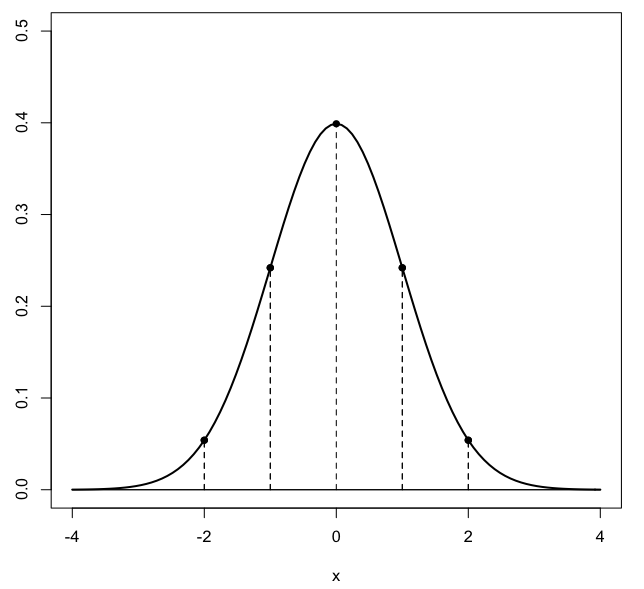
\includegraphics [scale=0.4] {gauss3.png} \end{center}

\title{Sequences}
\date{}

\begin{document}
\maketitle
\Large

A sequence is a list or ordered set of numbers $(a_1, a_2, a_3, \dots)$.

A sequence of numbers $(a_n)$ starts at a specific place, with a particular first term $a_1$ and then goes on forever.
\[ (a_n) = a_1,  a_2, a_3, \dots a_n, \dots \]
Usually, there will be some kind of pattern:

\[ 1,2,3 \dots \]
or 
\[ \frac{1}{2}, \ \frac{1}{4}, \ \frac{1}{8}, \dots \]

There is an important distinction between the notation for an individual term:  $a_n$, and the sequence itself:  $(a_n)$.

Technically a sequence in $\mathbb{R}$ is thought of as being a \emph{function} from the natural numbers to the reals ($f : \mathbb{N} \rightarrow \mathbb{R}$).

A sequence may be defined by a specific formula like $1/n$ or it may be described by a recurrence relation like $a_{n+2} = a_n + a_{n+1}$ (the Fibonacci numbers).  For a recurrence we must specify the first term (or first and second terms in the case of Fibonacci).

Consider
\[ a_{n+1} = \frac{a_n + 2/a_n}{2} \]
with $a_1 = 1$.
\[ (a_n) = 1, \frac{3}{2}, \frac{17}{12}, \frac{577}{408}, \frac{665857}{470832} \dots \] 
The last term shown is equal to $\sqrt{2}$ to $11$ places ($1.41421356237 \dots$).  This is not a coincidence!

or a last example:

\[ a_{n+1} = a_n + \frac{1}{n^2} = \frac{\pi^2}{6} \]

A sequence of random numbers would be a perfectly good sequence, but not much fun to work with.

\subsection*{monotonic sequences}
$\bullet$  The sequence ($a_n$) is \emph{increasing} $\iff \forall \ n \in \mathbb{N}, \ \ \ a_{n+1} \ge a_n$

This kind of formulation is very standard.  We specify $\forall \ n \in \mathbb{N}$, meaning every term of the sequence.  Or we might specify some particular $N \in \mathbb{N}$, and require that the indices for the particular terms be larger ($n > N$).

Note the $\ge$ in this example.  A monotonic increasing sequence is actually defined as not decreasing, so it can stay the same.  

\[ 5, \ 5, \ 5, \dots \]
is a monotonic sequence.

A more restrictive condition is to be \emph{strictly increasing}.

$\bullet$  A \emph{monotonic} sequence is either increasing or decreasing.

So there are two different types of monotonic sequences, those that do not go down and those that do not go up.  For the most part, monotonic sequences that are increasing are mirror images of the ones that decrease, and we can concentrate on the first class.

\subsection*{bounded sequences}

If we can find a number $M$ which is never exceeded by any term in the sequence, then it is bounded above.  

$\bullet$  The sequence ($a_n$) is \emph{bounded above} $\iff$
\[ \exists \ M \in \mathbb{R} \ | \ \forall \ n \in \mathbb{N}, a_n \le M \]

There is some $M$ such that for all terms in the sequence, those terms are smaller than $M$.

$\bullet$  Any sequence that has an upper bound has many upper bounds (if $M$ is an upper bound, then surely $M+1$ is also an upper bound).

$\bullet$  The sequence ($a_n$) is \emph{bounded} $\iff \exists \ M > 0 \ | \ \forall \ n \in \mathbb{N}, |a_n| \le M$  

A sequence is bounded if it is bounded above \emph{and} bounded below.
\begin{center} 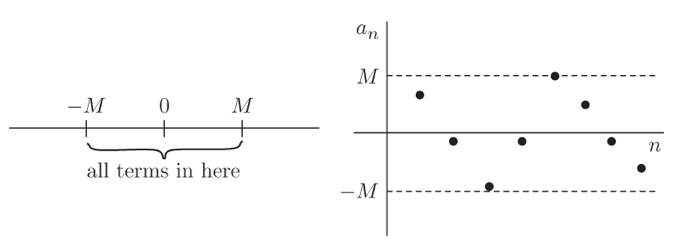
\includegraphics [scale=0.5] {bounded1.png} \end{center}

\subsection*{upper bound}

It's important that the sets we talk about not be empty.

An upper bound of a non-empty subset of $\mathbb{R}$ is an element $b \in \mathbb{R}$ such that $b \ge a$ for all $a \in \mathbf{A}$.

Suppose $\mathbf{A}$ consists of all $x \in \mathbb{R} \ | \ x < 0$.  Then $1$ is an upper bound for $\mathbf{A}$, but so is $2$ and so is $0$.

The reason for the restriction to non-empty subsets has to do with the definition of an upper bound.  The statement $b > a$ for every member $a \in \mathbf{A}$ is \emph{true} for any $b$ if $\mathbf{A}$ is empty ($\mathbf{A} = \varnothing$).

\subsection*{least upper bound}

$\bullet$  $u$ is an upper bound for $\mathbf{A}$ if $\forall \ x \in \mathbf{A}, x \le u$.

$\bullet$  $U$ least upper bound for $\mathbf{A}$ if for all upper bounds $u$, $U \le u$.

Note that for $U$ to be the least upper bound of $\mathbf{A}$, it is not necessary that $U \in \mathbf{A}$.

$\circ$  Example:  suppose $\mathbf{A}$ consists of all $x \in \mathbb{R} \ | \ x < 0$.  Then $0$ is the least upper bound of $\mathbf{A}$.

$0$ is the least upper bound of both $\{x \ | \ x < 0\}$ and $\{x \ | \ x \le 0\}$, but only in the second case is $0$ a member of the set.

The least upper bound of a subset of $\mathbb{R}$ is often called the \textbf{supremum} of the set, as in $\mathbf{sup}(\mathbf{A}) = 0$.  

If a non-empty set $\mathbf{A}$ has an upper bound, it has a least upper bound.

In our example above, $0$ is the least upper bound of $\mathbf{A}$.  $0$ is the \textbf{supremum} of the set of negative real numbers.

The supremum is not necessarily $\in \mathbf{A}$, but if it is then it is the maximum element of $\mathbf{A}$.

An epsilon-delta definition says:  if $\mathbf{A}$ is bounded above with $U = sup \ \mathbf{A}$ then
\[ \forall \ \epsilon > 0 \ \exists \ x \in  \mathbf{A} \ | \  x > U - \epsilon \]

There is no "last number" before the least upper bound.  No matter how small you make $\epsilon$, one can always find $x$ whose distance from $U$ is smaller than $\epsilon$.

No matter how small is $\epsilon$ we can always find a negative number closer to zero than that.

\subsection*{convergent sequences}
$\bullet$  The sequence ($a_n$) \emph{converges} to $a$  $\iff$
\[ \forall \ \epsilon > 0, \ \exists \ N \in \mathbb{N} \ | \ \forall \ n > N, |a_n - a| < \epsilon \]
\begin{center} 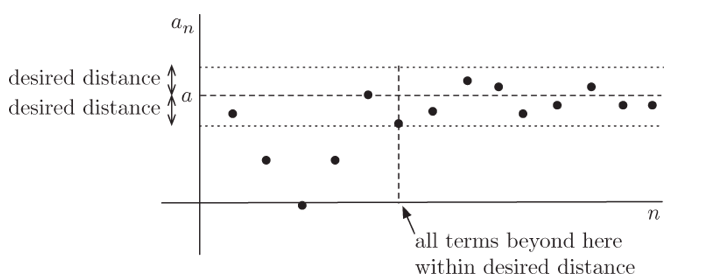
\includegraphics [scale=0.5] {convergent1.png} \end{center}

The early behavior of a sequence is irrelevant.  The requirement is that at some point (for index $n > N$), all the terms after $a_n$ must be closer than $\epsilon$ to the value $a$:  that is $|a_n - a| < \epsilon$.  The terms may be either $> a$ or $< a$.

$\epsilon$ can be chosen as small as we like, and the sequence must get as close as $\epsilon$ to the value $a$.

$\bullet$  Suppose that $(a_n)$ is a sequence and $L$ is a real number. If for all $\epsilon > 0$, we can find a term in the sequence such that it differs from $L$ by less than $\epsilon$ 
\[ |a_n - L | < \epsilon \]
and the same is true for all subsequent terms, then the sequence $(a_n)$ is \emph{convergent} and $L$ is its \emph{limit}.

A convergent sequence is bounded.  If a sequence is not bounded, then it is not convergent.

\subsection*{theorem}

$\bullet$ Any convergent sequence has a \emph{least upper bound} and a greatest lower bound.

\subsection*{proof 1}

Suppose that the sequence $(a_n) \rightarrow \alpha$.  Take $\epsilon = 1$.  Simply choose $N$ so that when $n > N$, we have $a_n$ within $1$ of $\alpha$.  ($|a_n - \alpha| < \epsilon = 1$).

Apart from the terms $(a_1, \dots a_N)$ we have that all the terms of the sequence are bounded by $\alpha + 1$ and $\alpha - 1$.  So an upper bound for the sequence is max$(a_1, \dots a_N, \alpha + 1)$.

\subsection*{Any convergent sequence is bounded}

$\bullet$  If $(a_n)$ is a sequence of real numbers that is convergent to $L \in \mathbb{R}$, that is, with $lim_{n \rightarrow \infty} \ a_n = L$, then $(a_n)$ is bounded.

The problem here is that we cannot take the maximum of an infinite set.  The idea of the proof is that, after some point in the sequence, all of the (infinite number of) terms in the sequence is within $L \pm \epsilon$.

\subsection*{proof 2}
For arbitrary $\epsilon$, by the definition of convergence there exists $N \in \mathbb{N}$ such that if $n \ge N$ then
\[ |a_n - L| < \epsilon \]
Let $\epsilon = 1$:
\[ |a_n - L| < 1 \]
\[ -1 < a_n - L < 1 \]
\[ L-1 < a_n < L+1 \]
\[ |a_n| < L + 1 \]

So now we know that a possible bound for $(a_n)$ is $L + 1$. Either that is true, or one of the terms before $a_N$ has a greater magnitude.  We set
\[ M = \text{max} \{|a_1|, |a_2|, \dots ,|a_{N-1}|, |L| + 1 \} \]

Therefore, for all $n \in N, |a_n| < M$ and so $(a_n)$ is bounded.

The converse is not true.  Consider
\[ (b_n) = (-1)^n = -1, \ 1, \ -1, \ 1 \dots \]
This sequence is bounded (since $|a_n| \le 1$ for all $n \in \mathbb{N}$), but it does not converge.

\end{document}